\section{Sets of Real Numbers and the Cartesian Coordinate Plane}

\subsection{Sets of Numbers}
\begin{definition}[Set]
    A \textbf{set} is a well-defined collection of objects which are called the 'elements' of the set. Here, 'well-defined' means that it is possible to determine if something belongs to the collection or not, without prejudice.
\end{definition}

\begin{definition}
    \textbf{Ways to describe sets}
    \begin{enumerate}
        \item \textbf{The Verbal Method}: Use a sentence to define a set.
        \item \textbf{The Roster Method}: Begin with a left brace '\{', list each element of the set only once and then end with a right brace '\}'.
        \item \textbf{The Set-Builder Method}: A combination of the verbal and roster methods using a "dummy variable" such as $x$.
    \end{enumerate}
\end{definition}

\begin{definition}
    \textbf{Sets of Numbers}
    \begin{enumerate}
        \item The \textbf{Empty Set}: $\emptyset = \{\} = \{x \mid x \neq x\}$. This is the set with no elements.
        \item The \textbf{Natural Numbers}: $\mathbb{N} = \{1,2,3,...\}$. The periods of ellipsis here indicate that the natural numbers contain 1, 2, 3, 'and so forth'.
        \item The \textbf{Whole Numbers}: $\mathbb{W} = \{0,1,2,...\}$
        \item The \textbf{Integers}: $\mathbb{Z} = \{...,-3,-2,-1,0,1,2,3,...\}$
        \item The \textbf{Rational Numbers}: $\mathbb{Q} = \{\frac{a}{b} \mid a \in \mathbb{Z} \land b \in \mathbb{Z}\}$. Rational numbers are the ratios of integers.
        \item The \textbf{Real Numbers}: $\mathbb{R} = \{x \mid x \text{ possesses a decimal representation.}\}$
        \item The \textbf{Irrational Numbers}: $\mathbb{P} = \{x \mid x \text{ is a non-rational real number.}\}$ Said another way, an irrational number is a decimal which neither repreats nor terminates.
        \item The \textbf{Complex Numbers}: $\mathbb{C} = \{a+bi \mid a, b \in \mathbb{R} \land i=\sqrt{-1}\}$.
    \end{enumerate}
\end{definition}

\begin{definition}[Intervals]
    Visualizing $\mathbb{R}$ as a line, segments on this line are called \textbf{intervals} of numbers.
    An interval can be described as a set in the form $\{x \mid a < x < b\}$, or in interval notation $(a, b)$
\end{definition}

\begin{definition}[Set Operations]
    Supposing that $A$ and $B$ are two sets.
    \begin{itemize}
        \item The \textbf{intersection} of $A$ and $B$: $A \cap B = \{x \mid x \in A \land x \in B\}$
        \item The \textbf{union} of $A$ and $B$: $A \cup B = \{x \mid x \in A \lor x \in B\}$
    \end{itemize}
\end{definition}

\begin{definition}[Cartesian Coordinate System]
    The \textbf{Cartesian Coordinate System} is a coordinate system that specifies each point on it uniquely by a pair of real numbers called coordinates. In a Cartesian Coordinate Plane:
    \begin{itemize}
        \item $(a, b)$ and $(c, d)$ represent the same point in the plane if and only if $a = c \land b = d$
        \item $(x, y)$ lies on the \textit{x-axis} if and only if $y = 0$
        \item $(x, y)$ lies on the \textit{y-axis} if and only if $x = 0$
        \item The origin is the point $(0,0)$. It is the only point common to both axes.
    \end{itemize}
\end{definition}

\begin{definition}[Symmmetry]
    Two points $(a, b)$ and $(c,d)$ in the plane are said to be:
    \begin{itemize}
        \item \textbf{symmetric about the \textit{x-axis}} if $a=c \land b = -d$
        \item \textbf{symmetric about the \textit{y-axis}} if $a=-c \land b = d$
        \item \textbf{symmetric about the \textit{origin}} if $a= -c \land b = -d$
    \end{itemize}
\end{definition}

\begin{definition}[Reflections]
    To reflect a point $(x, y)$ about the:
    \begin{itemize}
        \item \textit{x-axis}, replace $y$ with $-y$
        \item \textit{y-axis}, replace $x$ with $-x$
        \item \textit{origin}, replace $x$ with $-x$ and $y$ with $-y$
    \end{itemize}
\end{definition}

\begin{definition}[Distance]
    Supposing we hace two points $P(x_0,y_0)$ and $Q(x_1,y_1)$ in the plane. The \textbf{distance} between $P$ and $Q$ is the length of the line segment joining $P$ with $Q$. Using the pythagorean theorem we can derive the distance formula as:
    \[
        d = \sqrt{(x_1-x_0)^2 + (y_1-y_0)^2}
    \]
\end{definition}

\begin{definition}
    The midpoint $M$ of the line segment connecting $P(x_0,y_0)$ and $Q(x_1,y_1)$ is:
    \[
        M = (\frac{x_0+x_1}{2}, \frac{y_0+y_1}{2})
    \]
\end{definition}


\subsection{Problems}
\begin{enumerate}
    \item [2.] $(-1,5] \cap [0, 8) = [0, 5]$

    \item [8.] $(-\infty, 5) \cup (5, \infty)$

    \item [20.] \leavevmode
          \begin{center}
              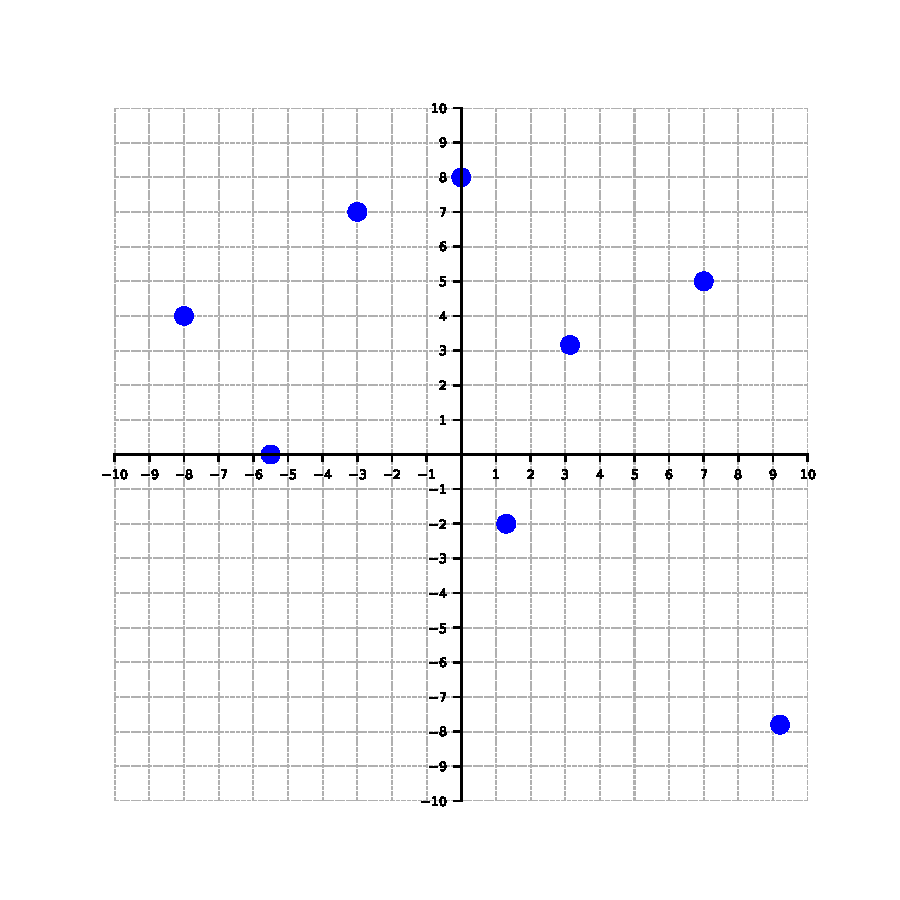
\includegraphics[width=0.5\textwidth]{figures/01/01/exercise_20.pdf}
          \end{center}

    \item [22.]
          \[ d = \sqrt{(-3-1)^2 + (5-2)^2} = \sqrt{16 + 9} = \sqrt{25} = 5\]
          \[M = (\frac{1-3}{2}, \frac{2+5}{2}) = (-1, 3.5)\]

    \item [30.]
          \[4 = \sqrt{(3-x)^2 + (2+1)^2} = \sqrt{9-6x+x^2 + 9} = \sqrt{x^2-6x+18}\]
          \[x^2-6x+18=16\]
          \[x^2-6x+2=0\]
          \[x_1 = 3 + \sqrt{7}, x_2 = 3-\sqrt{7}\]
          \[(3+\sqrt{7}, -1), (3-\sqrt{7}, -1)\]

    \item [34.] He's at $(-3,-4)$, at a distance of $5$ miles, after running he will be at $(4,-4)$

    \item [35.]
          \begin{enumerate}
              \item
                    \[d = \sqrt{(a-a)^2 + (y_1 - y_0)^2} = \sqrt{(y_1 - y_0)^2} = y_1 - y_0\]
              \item
                    \[d = \sqrt{(x_1 - x_0)^2 + (b-b)^2} = \sqrt{(x_1 - x_0)^2} = x_1 - x_0\]
              \item
                    \[d = \sqrt{(x-x)^2 + (y-y)^2} = \sqrt{0} = 0\]
          \end{enumerate}

    \item [36.]
          \[M = (\frac{x_1 + x_2}{2}, \frac{y_1 + y_2}{2})\]
          \begin{align*}
              d_{PM} & = \sqrt{(\frac{x_1 + x_2}{2} - x_1)^2 + (\frac{y_1 + y_2}{2} - y_1)^2} \\
                     & = \sqrt{(\frac{x_2-x_1}{2})^2 + (\frac{y_2-y_1}{2})^2}                 \\
                     & = \sqrt{\frac{x_1^2-2x_1x_2+x_2^2}{4} + \frac{y_1^2-2y_1y_2+y_2^2}{4}} \\
              d_{QM} & = \sqrt{(\frac{x_1 + x_2}{2} - x_2)^2 + (\frac{y_1 + y_2}{2} - y_2)^2} \\
                     & = \sqrt{(\frac{x_1-x_2}{2})^2 + (\frac{y_1-y_2}{2})^2}                 \\
                     & = \sqrt{\frac{x_1^2-2x_1x_2+x_2^2}{4} + \frac{y_1^2-2y_1y_2+y_2^2}{4}}
          \end{align*}
          \[d_{PM} = d_{QM}\]

    \item [37.] To prove that the points are the vertices of a right triangle there must be an internal angle with a value of 90deg or prove the converse of the pythagorean theorem.
          \begin{enumerate}
              \item
                    \[AB = \sqrt{13}, AC=2\sqrt{13}, BC=\sqrt{65}\]
                    \[BC^2 = 65 = AB^2 + AC^2 = 13 + 52\]
              \item
                    \[AB = 5\sqrt{2}, AC=5, BC=5\]
                    \[AB^2 = 50 = AC^2 + BC^2 = 25 + 25\]
          \end{enumerate}

    \item [38.] To find the remaining point that makes the square, we must find a point that is at the same distance as the other points. We can create a vector from one of the sides of the square and just use it as a base to create the square.
          If we take $CB=(4,3)$, then applying that to A, we get $D=(1, 4)$

\end{enumerate}